% Options for packages loaded elsewhere
\PassOptionsToPackage{unicode}{hyperref}
\PassOptionsToPackage{hyphens}{url}
%
\documentclass[
]{article}
\usepackage{amsmath,amssymb}
\usepackage{lmodern}
\usepackage{iftex}
\ifPDFTeX
  \usepackage[T1]{fontenc}
  \usepackage[utf8]{inputenc}
  \usepackage{textcomp} % provide euro and other symbols
\else % if luatex or xetex
  \usepackage{unicode-math}
  \defaultfontfeatures{Scale=MatchLowercase}
  \defaultfontfeatures[\rmfamily]{Ligatures=TeX,Scale=1}
\fi
% Use upquote if available, for straight quotes in verbatim environments
\IfFileExists{upquote.sty}{\usepackage{upquote}}{}
\IfFileExists{microtype.sty}{% use microtype if available
  \usepackage[]{microtype}
  \UseMicrotypeSet[protrusion]{basicmath} % disable protrusion for tt fonts
}{}
\makeatletter
\@ifundefined{KOMAClassName}{% if non-KOMA class
  \IfFileExists{parskip.sty}{%
    \usepackage{parskip}
  }{% else
    \setlength{\parindent}{0pt}
    \setlength{\parskip}{6pt plus 2pt minus 1pt}}
}{% if KOMA class
  \KOMAoptions{parskip=half}}
\makeatother
\usepackage{xcolor}
\usepackage[margin=1in]{geometry}
\usepackage{color}
\usepackage{fancyvrb}
\newcommand{\VerbBar}{|}
\newcommand{\VERB}{\Verb[commandchars=\\\{\}]}
\DefineVerbatimEnvironment{Highlighting}{Verbatim}{commandchars=\\\{\}}
% Add ',fontsize=\small' for more characters per line
\usepackage{framed}
\definecolor{shadecolor}{RGB}{248,248,248}
\newenvironment{Shaded}{\begin{snugshade}}{\end{snugshade}}
\newcommand{\AlertTok}[1]{\textcolor[rgb]{0.94,0.16,0.16}{#1}}
\newcommand{\AnnotationTok}[1]{\textcolor[rgb]{0.56,0.35,0.01}{\textbf{\textit{#1}}}}
\newcommand{\AttributeTok}[1]{\textcolor[rgb]{0.77,0.63,0.00}{#1}}
\newcommand{\BaseNTok}[1]{\textcolor[rgb]{0.00,0.00,0.81}{#1}}
\newcommand{\BuiltInTok}[1]{#1}
\newcommand{\CharTok}[1]{\textcolor[rgb]{0.31,0.60,0.02}{#1}}
\newcommand{\CommentTok}[1]{\textcolor[rgb]{0.56,0.35,0.01}{\textit{#1}}}
\newcommand{\CommentVarTok}[1]{\textcolor[rgb]{0.56,0.35,0.01}{\textbf{\textit{#1}}}}
\newcommand{\ConstantTok}[1]{\textcolor[rgb]{0.00,0.00,0.00}{#1}}
\newcommand{\ControlFlowTok}[1]{\textcolor[rgb]{0.13,0.29,0.53}{\textbf{#1}}}
\newcommand{\DataTypeTok}[1]{\textcolor[rgb]{0.13,0.29,0.53}{#1}}
\newcommand{\DecValTok}[1]{\textcolor[rgb]{0.00,0.00,0.81}{#1}}
\newcommand{\DocumentationTok}[1]{\textcolor[rgb]{0.56,0.35,0.01}{\textbf{\textit{#1}}}}
\newcommand{\ErrorTok}[1]{\textcolor[rgb]{0.64,0.00,0.00}{\textbf{#1}}}
\newcommand{\ExtensionTok}[1]{#1}
\newcommand{\FloatTok}[1]{\textcolor[rgb]{0.00,0.00,0.81}{#1}}
\newcommand{\FunctionTok}[1]{\textcolor[rgb]{0.00,0.00,0.00}{#1}}
\newcommand{\ImportTok}[1]{#1}
\newcommand{\InformationTok}[1]{\textcolor[rgb]{0.56,0.35,0.01}{\textbf{\textit{#1}}}}
\newcommand{\KeywordTok}[1]{\textcolor[rgb]{0.13,0.29,0.53}{\textbf{#1}}}
\newcommand{\NormalTok}[1]{#1}
\newcommand{\OperatorTok}[1]{\textcolor[rgb]{0.81,0.36,0.00}{\textbf{#1}}}
\newcommand{\OtherTok}[1]{\textcolor[rgb]{0.56,0.35,0.01}{#1}}
\newcommand{\PreprocessorTok}[1]{\textcolor[rgb]{0.56,0.35,0.01}{\textit{#1}}}
\newcommand{\RegionMarkerTok}[1]{#1}
\newcommand{\SpecialCharTok}[1]{\textcolor[rgb]{0.00,0.00,0.00}{#1}}
\newcommand{\SpecialStringTok}[1]{\textcolor[rgb]{0.31,0.60,0.02}{#1}}
\newcommand{\StringTok}[1]{\textcolor[rgb]{0.31,0.60,0.02}{#1}}
\newcommand{\VariableTok}[1]{\textcolor[rgb]{0.00,0.00,0.00}{#1}}
\newcommand{\VerbatimStringTok}[1]{\textcolor[rgb]{0.31,0.60,0.02}{#1}}
\newcommand{\WarningTok}[1]{\textcolor[rgb]{0.56,0.35,0.01}{\textbf{\textit{#1}}}}
\usepackage{graphicx}
\makeatletter
\def\maxwidth{\ifdim\Gin@nat@width>\linewidth\linewidth\else\Gin@nat@width\fi}
\def\maxheight{\ifdim\Gin@nat@height>\textheight\textheight\else\Gin@nat@height\fi}
\makeatother
% Scale images if necessary, so that they will not overflow the page
% margins by default, and it is still possible to overwrite the defaults
% using explicit options in \includegraphics[width, height, ...]{}
\setkeys{Gin}{width=\maxwidth,height=\maxheight,keepaspectratio}
% Set default figure placement to htbp
\makeatletter
\def\fps@figure{htbp}
\makeatother
\setlength{\emergencystretch}{3em} % prevent overfull lines
\providecommand{\tightlist}{%
  \setlength{\itemsep}{0pt}\setlength{\parskip}{0pt}}
\setcounter{secnumdepth}{-\maxdimen} % remove section numbering
\newlength{\cslhangindent}
\setlength{\cslhangindent}{1.5em}
\newlength{\csllabelwidth}
\setlength{\csllabelwidth}{3em}
\newlength{\cslentryspacingunit} % times entry-spacing
\setlength{\cslentryspacingunit}{\parskip}
\newenvironment{CSLReferences}[2] % #1 hanging-ident, #2 entry spacing
 {% don't indent paragraphs
  \setlength{\parindent}{0pt}
  % turn on hanging indent if param 1 is 1
  \ifodd #1
  \let\oldpar\par
  \def\par{\hangindent=\cslhangindent\oldpar}
  \fi
  % set entry spacing
  \setlength{\parskip}{#2\cslentryspacingunit}
 }%
 {}
\usepackage{calc}
\newcommand{\CSLBlock}[1]{#1\hfill\break}
\newcommand{\CSLLeftMargin}[1]{\parbox[t]{\csllabelwidth}{#1}}
\newcommand{\CSLRightInline}[1]{\parbox[t]{\linewidth - \csllabelwidth}{#1}\break}
\newcommand{\CSLIndent}[1]{\hspace{\cslhangindent}#1}

\usepackage{tcolorbox}

\definecolor{mybluebackground}{HTML}{e7f3fe}
\definecolor{mybluecolor}{HTML}{31708f}
\definecolor{myblueborder}{HTML}{bce8f1}
\definecolor{mybrownbackground}{HTML}{f9f0e4}
\definecolor{mybrowncolor}{HTML}{8a6d3b}
\definecolor{mybrownborder}{HTML}{faebcc}

\newtcolorbox{infobox}{
  colback=mybluebackground,
  colframe=myblueborder,
  coltext=mybluecolor,
  boxsep=3pt,
  boxrule=1pt,
  arc=4pt}

\newtcolorbox{warningbox}{
  colback=mybrownbackground,
  colframe=mybrownborder,
  coltext=mybrowncolor,
  boxsep=3pt,
  boxrule=1pt,
  arc=4pt}

\usepackage{amsmath}
\usepackage{booktabs}
\usepackage{float}
\usepackage{subcaption}
\usepackage{caption}
\floatplacement{figure}{H}
\usepackage{booktabs}
\usepackage{longtable}
\usepackage{array}
\usepackage{multirow}
\usepackage{wrapfig}
\usepackage{float}
\usepackage{colortbl}
\usepackage{pdflscape}
\usepackage{tabu}
\usepackage{threeparttable}
\usepackage{threeparttablex}
\usepackage[normalem]{ulem}
\usepackage{makecell}
\usepackage{xcolor}
\ifLuaTeX
  \usepackage{selnolig}  % disable illegal ligatures
\fi
\IfFileExists{bookmark.sty}{\usepackage{bookmark}}{\usepackage{hyperref}}
\IfFileExists{xurl.sty}{\usepackage{xurl}}{} % add URL line breaks if available
\urlstyle{same} % disable monospaced font for URLs
\hypersetup{
  pdftitle={Mapping species distribution, richness and endemism},
  pdfauthor={Ian Ondo},
  hidelinks,
  pdfcreator={LaTeX via pandoc}}

\title{Mapping species distribution, richness and endemism}
\author{Ian Ondo}
\date{2023-07-24}

\begin{document}
\maketitle

{
\setcounter{tocdepth}{2}
\tableofcontents
}
\begin{warningbox}

\textbf{Package notes:}\\
We need to install the following set of R packages to successfully run
the codes in this vignette:

\begin{itemize}
\tightlist
\item
  \textbf{rsdm} (Dowle and Srinivasan 2021)
\item
  \textbf{terra} (Hijmans 2023)
\item
  \textbf{ggplot2} (Wickham 2016)
\item
  \textbf{ggpubr} (Kassambara 2023)
\end{itemize}

\end{warningbox}

\hypertarget{introduction}{%
\section{Introduction}\label{introduction}}

In this vignette, we will demonstrate how to build a species richness
and endemism map based on species probability of occurrence (Crisp et
al. 2001; Calabrese et al. 2014).\\
The grid-level species richness \(S_j\) prediction at the \(j^{th}\)
grid cell location follows a Poisson binomial distribution (Calabrese et
al. 2014), meaning that the expected value (mean) and variance of
stacking the probability of occurrence of \emph{K} species is given by:

\begin{gather}
\tag{1}
E(S_j) = \sum_{k=1}^Kp_{j,k}
\\
\tag{2}
Var(S_j) = \sum_{k=1}^K(1-p_{j,k})p_{j,k}
\end{gather}

Where, \(p_{j,k}\) is the probability of occurrence of species \emph{k}
in grid cell \emph{j}.

The grid-level endemism (hereafter called \emph{weighted endemism})
\(WE_j\) prediction at \emph{j} is computed as the species richness
\(S_j\) weighted by the inverse of the range size of species (Crisp et
al. 2001):

\begin{gather}
\tag{3}
WE_j = \sum_{k=1}^K(p_{j,k}\times\frac{1}{Range Size_k})
\\
\tag{4}
RangeSize_k = \sum_{j=1}^{J_k}p_{j,k}
\end{gather}

Where, \(J_k\) is the number of grid cells species \emph{k} is predicted
to occur in.

\hypertarget{step-1-obtaining-species-probability-of-occurrence-datamaps}{%
\section{Step 1: Obtaining species probability of occurrence
data/maps}\label{step-1-obtaining-species-probability-of-occurrence-datamaps}}

If you do not have probability maps of species occurrences yet, please
have a look at the vignette
\href{}{\textbf{\textcolor{black}{\underline{Modelling species distribution}}}}
to obtain such maps using the package \textbf{rsdm}.\\
Here, we are going to use the outputs of the modelling of Pironon S.
(2023), which can be downloaded from its Zenodo repository at
\href{https://doi.org/10.5281/zenodo.8176318}{\textbf{https://doi.org/10.5281/zenodo.8176318}}.
Download the dataset, unzip it and save the file
\texttt{species\_proba\_per\_cell.rds} somewhere on your computer, then
load it into R:

\begin{Shaded}
\begin{Highlighting}[]

\CommentTok{\# load the distribution object (this may take a while, so be patient!)}
\NormalTok{species\_proba\_per\_cell }\OtherTok{\textless{}{-}} \FunctionTok{readRDS}\NormalTok{(}\StringTok{\textquotesingle{}path/to/species\_proba\_per\_cell.rds\textquotesingle{}}\NormalTok{) }
\NormalTok{data.table}\SpecialCharTok{::}\FunctionTok{setkey}\NormalTok{(species\_proba\_per\_cell, species) }\CommentTok{\# enable fast binary search of species}

\NormalTok{species\_proba\_per\_cell}
\end{Highlighting}
\end{Shaded}

It is a R Data Serialization (RDS) file containing a data.table object
with three columns:

\begin{itemize}
\tightlist
\item
  species: index number of the species
\item
  proba: species occurrence probability
\item
  cell: raster grid cell number
\end{itemize}

The index number ranges between 1 and 35687 and refers to the position
of the species in the list of useful plants when sorted in alphabetic
order. The species occurrence probability ranges between 0 and 1, and
the grid cell number between 1 and 2251762 (i.e.~up to the total number
of grid cells that contain the global raster layers of environmental
predictors used to model the species).

We are going to use the list of useful plants and an environmental
raster layer used in Pironon S. (2023) to select and map the
distribution of \emph{Acacia cowleana}

\begin{Shaded}
\begin{Highlighting}[]

\CommentTok{\# select the species you would like to get the distribution for }
\NormalTok{my\_species\_ID  }\OtherTok{\textless{}{-}}\NormalTok{ UsefulPlants}\SpecialCharTok{:::}\NormalTok{usefulplants }\SpecialCharTok{|\textgreater{}} \CommentTok{\# list of useful plants }
\NormalTok{  dplyr}\SpecialCharTok{::}\FunctionTok{mutate}\NormalTok{(}\AttributeTok{ID=}\NormalTok{dplyr}\SpecialCharTok{::}\FunctionTok{row\_number}\NormalTok{()) }\SpecialCharTok{|\textgreater{}} \CommentTok{\# calculate a row id}
\NormalTok{  dplyr}\SpecialCharTok{::}\FunctionTok{filter}\NormalTok{(binomial\_acc\_name}\SpecialCharTok{==}\StringTok{"Acacia cowleana"}\NormalTok{) }\SpecialCharTok{|\textgreater{}}  \CommentTok{\# select Acacia cowleana}
\NormalTok{  dplyr}\SpecialCharTok{::}\FunctionTok{pull}\NormalTok{(ID) }\CommentTok{\# extract its row index number}

\CommentTok{\# extract the species probability of occurrence   }
\NormalTok{my\_species\_probas }\OtherTok{\textless{}{-}}\NormalTok{ species\_proba\_per\_cell[}\FunctionTok{J}\NormalTok{(my\_species\_ID)]}

\CommentTok{\# get valid cell numbers (i.e. cells with values)}
\NormalTok{valid.cells }\OtherTok{\textless{}{-}} \SpecialCharTok{!}\FunctionTok{is.na}\NormalTok{(my\_species\_probas[[}\StringTok{\textquotesingle{}cell\textquotesingle{}}\NormalTok{]])}

\CommentTok{\# create an empty raster }
\NormalTok{rast\_ref }\OtherTok{\textless{}{-}}\NormalTok{ terra}\SpecialCharTok{::}\FunctionTok{rast}\NormalTok{(}\FunctionTok{system.file}\NormalTok{(}\StringTok{"extdata"}\NormalTok{,}\StringTok{"sdm\_env\_raster\_layers.tif"}\NormalTok{,}
                                    \AttributeTok{package=}\StringTok{"UsefulPlants"}\NormalTok{))[[}\DecValTok{1}\NormalTok{]]}
\NormalTok{my\_species\_distribution }\OtherTok{\textless{}{-}}\NormalTok{ rast\_ref}

\CommentTok{\# make sure to mask out the original values}
\NormalTok{terra}\SpecialCharTok{::}\FunctionTok{values}\NormalTok{(my\_species\_distribution) }\OtherTok{\textless{}{-}} \ConstantTok{NA} 

\CommentTok{\# fill up raster values with corresponding estimates}
\NormalTok{my\_species\_distribution[my\_species\_probas[[}\StringTok{\textquotesingle{}cell\textquotesingle{}}\NormalTok{]][valid.cells]] }\OtherTok{\textless{}{-}} 
\NormalTok{  my\_species\_probas[[}\StringTok{\textquotesingle{}proba\textquotesingle{}}\NormalTok{]][valid.cells]}

\CommentTok{\# optionally restrict the map extent to fit the species distribution and save the results}
\NormalTok{ext }\OtherTok{\textless{}{-}}\NormalTok{ raster}\SpecialCharTok{::}\FunctionTok{rasterFromCells}\NormalTok{(raster}\SpecialCharTok{::}\FunctionTok{raster}\NormalTok{(my\_species\_distribution), }
\NormalTok{                               my\_species\_probas[[}\StringTok{\textquotesingle{}cell\textquotesingle{}}\NormalTok{]][valid.cells], }\AttributeTok{values=}\ConstantTok{FALSE}\NormalTok{) }\SpecialCharTok{|\textgreater{}}
\NormalTok{  terra}\SpecialCharTok{::}\FunctionTok{extend}\NormalTok{(}\FunctionTok{c}\NormalTok{(}\DecValTok{2}\NormalTok{,}\DecValTok{2}\NormalTok{)) }\CommentTok{\# extend with a number of rows and columns (2 at each side)}
\NormalTok{terra}\SpecialCharTok{::}\FunctionTok{crop}\NormalTok{(my\_species\_distribution, terra}\SpecialCharTok{::}\FunctionTok{rast}\NormalTok{(ext), }
            \AttributeTok{filename=}\StringTok{"Acacia\_cowleana.tif"}\NormalTok{, }
            \AttributeTok{overwrite=}\ConstantTok{TRUE}\NormalTok{)}

\CommentTok{\# or save directly your map using the global extent}
\NormalTok{terra}\SpecialCharTok{::}\FunctionTok{writeRaster}\NormalTok{(my\_species\_distribution, }\StringTok{"Acacia\_cowleana.tif"}\NormalTok{, }\AttributeTok{overwrite=}\ConstantTok{TRUE}\NormalTok{)}
\end{Highlighting}
\end{Shaded}

\hypertarget{step-2-aggregating-probability-maps}{%
\section{Step 2: Aggregating probability
maps}\label{step-2-aggregating-probability-maps}}

If we are interested in species richness patterns, we must aggregate a
collection of raster maps usually derived at different geographic
extents because of the differences in the spatial coverage of species
distribution. One solution is re-use the reference raster \(rast_{ref}\)
encompassing the total geographic extent of all species distribution
maps, e.g.~a worldwide raster map, extract the grid cells in
\(rast_{ref}\) that overlap with each species probability map and
retrieve the corresponding species occurrence probabilities.\\
Let's assume that following \textbf{Step 1}, we stored our species
probability maps predictions in a folder named
``\texttt{usefulplants\_rast\_maps}'', then:

\begin{Shaded}
\begin{Highlighting}[]

\CommentTok{\# get the list of raster maps files}
\NormalTok{rast\_list\_files }\OtherTok{=}\FunctionTok{list.files}\NormalTok{(}\StringTok{"\textasciitilde{}/usefulplants\_rast\_maps"}\NormalTok{,}
                              \CommentTok{\# replace .tif by the correct file extension}
                              \AttributeTok{pattern=}\StringTok{"}\SpecialCharTok{\textbackslash{}\textbackslash{}}\StringTok{.tif$"}\NormalTok{,}
                              \AttributeTok{full.names=}\NormalTok{T)}
\DocumentationTok{\#\# make sure that raster\textquotesingle{}s names correspond to species names !!}

\CommentTok{\# create a function that will extract cell numbers from the reference raster}
\CommentTok{\# and the individual maps predicted probabilities}
\NormalTok{get\_grid\_cell\_prob }\OtherTok{\textless{}{-}} \ControlFlowTok{function}\NormalTok{(k,ref)\{}
  \CommentTok{\# read the probability maps in memory}
\NormalTok{  r }\OtherTok{\textless{}{-}}\NormalTok{ raster}\SpecialCharTok{::}\FunctionTok{raster}\NormalTok{(k)}
  \CommentTok{\# extract cells with values}
  \CommentTok{\# (we could also select cells with values\textgreater{}0 to speed up the computations)}
\NormalTok{  vals }\OtherTok{\textless{}{-}}\NormalTok{ raster}\SpecialCharTok{::}\FunctionTok{values}\NormalTok{(r)}
\NormalTok{  cells }\OtherTok{\textless{}{-}} \FunctionTok{which}\NormalTok{(}\SpecialCharTok{!}\FunctionTok{is.na}\NormalTok{(vals))}
  \CommentTok{\# get the position of the species in the list of species maps files}
  \CommentTok{\# using the raster\textquotesingle{}s name and a out{-}of{-}scope vector of species names }
  \CommentTok{\# defined later}
\NormalTok{  species\_idx }\OtherTok{=} \FunctionTok{match}\NormalTok{(}\FunctionTok{gsub}\NormalTok{(}\StringTok{"\_"}\NormalTok{,}\StringTok{" "}\NormalTok{, }\FunctionTok{gsub}\NormalTok{(}\StringTok{"}\SpecialCharTok{\textbackslash{}\textbackslash{}}\StringTok{."}\NormalTok{,}\StringTok{"{-}"}\NormalTok{,}\FunctionTok{names}\NormalTok{(r))), sp.names)}
  \CommentTok{\# get cells in reference raster ref}
\NormalTok{  cells\_ref }\OtherTok{\textless{}{-}}\NormalTok{ raster}\SpecialCharTok{::}\FunctionTok{cellFromXY}\NormalTok{(ref, raster}\SpecialCharTok{::}\FunctionTok{xyFromCell}\NormalTok{(r,cells))}
  \CommentTok{\# returns a data.table }
\NormalTok{  data.table}\SpecialCharTok{::}\FunctionTok{data.table}\NormalTok{(}\AttributeTok{species=}\NormalTok{species\_idx,}
                                \AttributeTok{cell=}\NormalTok{cells\_ref,}
                                \AttributeTok{proba=}\NormalTok{r[cells])}
\NormalTok{\}}

\CommentTok{\# path to your reference raster. Make sure this raster has the same geographic }
\CommentTok{\# projection and resolution as your probability maps. It can be, for example, }
\CommentTok{\# one of the environmental raster layer used to predict your species probability}
\CommentTok{\# of occurrence.}
\NormalTok{rast\_ref\_file }\OtherTok{\textless{}{-}} \StringTok{"\textless{}path/to/reference/raster.tif\textgreater{}"} 

\CommentTok{\# split the vector of files paths into 100 chunks for parallel processing}
\NormalTok{raster\_split\_list }\OtherTok{\textless{}{-}}\NormalTok{ rsdm}\SpecialCharTok{::}\FunctionTok{chunk2}\NormalTok{(rast\_list\_files, }\DecValTok{100}\NormalTok{)}

\CommentTok{\# create a vector of species names}
\NormalTok{sp.names }\OtherTok{\textless{}{-}} \FunctionTok{gsub}\NormalTok{(}\StringTok{"\_"}\NormalTok{,}\StringTok{" "}\NormalTok{,rsdm}\SpecialCharTok{::}\FunctionTok{strip\_extension}\NormalTok{(}\FunctionTok{basename}\NormalTok{(rast\_list\_files)))}

\CommentTok{\# run function in parallel}
\CommentTok{\# foreach will copy all R objects in Global Environment within child processes,}
\CommentTok{\# so be careful to not store big objects in your environment !}
\NormalTok{doParallel}\SpecialCharTok{::}\FunctionTok{registerDoParallel}\NormalTok{(parallel}\SpecialCharTok{::}\FunctionTok{detectCores}\NormalTok{()}\SpecialCharTok{{-}}\DecValTok{1}\NormalTok{)}
\NormalTok{started.at}\OtherTok{=}\FunctionTok{proc.time}\NormalTok{()}
\NormalTok{species\_proba\_per\_cell }\OtherTok{\textless{}{-}}\NormalTok{ foreach}\SpecialCharTok{::}\FunctionTok{foreach}\NormalTok{(}\AttributeTok{k=}\NormalTok{raster\_split\_list,}
                                              \AttributeTok{.packages=}\FunctionTok{c}\NormalTok{(}\StringTok{"data.table"}\NormalTok{,}\StringTok{"raster"}\NormalTok{),}
                                              \AttributeTok{.combine=}\StringTok{\textquotesingle{}rbind\textquotesingle{}}\NormalTok{) }\SpecialCharTok{\%dopar\%}\NormalTok{ \{}
  \FunctionTok{gc}\NormalTok{()}
  \CommentTok{\# apply the function "get\_grid\_cell\_prob" to the set of raster maps k}
\NormalTok{  l }\OtherTok{\textless{}{-}} \FunctionTok{lapply}\NormalTok{(k, get\_grid\_cell\_prob, }\AttributeTok{ref=}\NormalTok{raster}\SpecialCharTok{::}\FunctionTok{raster}\NormalTok{(rast\_ref\_file))}
  \CommentTok{\# bind outputs and return}
  \FunctionTok{rbindlist}\NormalTok{(l,}\AttributeTok{fill=}\ConstantTok{TRUE}\NormalTok{)}
\NormalTok{\}}
\NormalTok{doParallel}\SpecialCharTok{::}\FunctionTok{stopImplicitCluster}\NormalTok{()}
\NormalTok{finished.at}\OtherTok{=}\FunctionTok{proc.time}\NormalTok{()}
\NormalTok{time\_taken }\OtherTok{\textless{}{-}}\NormalTok{ finished.at }\SpecialCharTok{{-}}\NormalTok{ started.at }\CommentTok{\# calculate amount of time elapsed}
\FunctionTok{cat}\NormalTok{(}
  \FunctionTok{sprintf}\NormalTok{(}\StringTok{"}\SpecialCharTok{\textbackslash{}n}\StringTok{ \textgreater{} End of computations ( Time elapsed : \%g hr \%g min \%g sec. )}\SpecialCharTok{\textbackslash{}n\textbackslash{}n}\StringTok{"}\NormalTok{,}
          \FunctionTok{as.vector}\NormalTok{(time\_taken[}\StringTok{\textquotesingle{}elapsed\textquotesingle{}}\NormalTok{])}\SpecialCharTok{/}\DecValTok{3600}\NormalTok{, }\FunctionTok{as.vector}\NormalTok{(time\_taken[}\StringTok{\textquotesingle{}elapsed\textquotesingle{}}\NormalTok{])}\SpecialCharTok{/}\DecValTok{60}\NormalTok{,}
          \FunctionTok{as.vector}\NormalTok{(time\_taken[}\StringTok{\textquotesingle{}elapsed\textquotesingle{}}\NormalTok{])))}
\NormalTok{rsdm}\SpecialCharTok{::}\FunctionTok{unregister}\NormalTok{()}

\CommentTok{\# make sure that probabilities lie between 0 and 1}
\NormalTok{species\_proba\_per\_cell[,proba}\SpecialCharTok{:}\ErrorTok{=}\FunctionTok{pmin}\NormalTok{(}\FunctionTok{pmax}\NormalTok{(proba, }\DecValTok{0}\NormalTok{, }\AttributeTok{na.rm=}\NormalTok{T), }\DecValTok{1}\NormalTok{, }\AttributeTok{na.rm=}\NormalTok{T)]}

\CommentTok{\# save the data.table in a rds file for later processing}
\CommentTok{\# (this may take a while !)}
\FunctionTok{saveRDS}\NormalTok{(species\_proba\_per\_cell, }\FunctionTok{file.path}\NormalTok{(}\FunctionTok{getwd}\NormalTok{(),}\StringTok{"species\_proba\_per\_cell.rds"}\NormalTok{))}
\end{Highlighting}
\end{Shaded}

\begin{warningbox}
\textbf{Important note:}

The method that we used to retrieve cells that overlap between the
reference and a probability raster only works if
\underline{the two raster grids are aligned}.\\
If they don't, this can be done by snapping the lower left corner and
upper right corner of the raster we want to aligned to the lower left
corner and upper right corner respectively of the nearest cell in the
snap raster (i.e.~reference raster).\\
The \textbf{snapRaster} function included in the \emph{Spatial Analyst}
extension of ArcGIS can be used to generate probability maps
\emph{snapped} to the reference map.

\end{warningbox}

\hypertarget{step-3-computing-the-species-richness-sr-and-its-standard-deviation-sd}{%
\section{\texorpdfstring{Step 3: Computing the species richness
\emph{SR} and its standard deviation
\emph{SD}}{Step 3: Computing the species richness SR and its standard deviation SD}}\label{step-3-computing-the-species-richness-sr-and-its-standard-deviation-sd}}

We just need to apply equations (1) and (2) on the \texttt{data.table}
object \texttt{species\_proba\_per\_cell}, but instead of computing the
variance at each grid cell \emph{j}, we are going to compute the
standard deviation \emph{SD} as follows:
\(SD(S_j)=\sqrt{\frac{Var(S_j)}{N}}=\sqrt{\frac{\sum_{k=1}^K(1-p_{j,k})p_{j,k}}{N}}\),
where N is the number of predicted values in \emph{j}.

\begin{Shaded}
\begin{Highlighting}[]

\CommentTok{\# load the species probabilities per grid cell data.table (if not done yet)}
\NormalTok{species\_proba\_per\_cell }\OtherTok{\textless{}{-}} \FunctionTok{readRDS}\NormalTok{(}\FunctionTok{file.path}\NormalTok{(}\FunctionTok{getwd}\NormalTok{(),}\StringTok{"species\_proba\_per\_cell.rds"}\NormalTok{))}

\CommentTok{\# compute species richness SR and its standard deviation SD using equation 1 and 2}
\NormalTok{species\_richness}\OtherTok{\textless{}{-}}\NormalTok{species\_proba\_per\_cell[,}\FunctionTok{list}\NormalTok{(}\AttributeTok{SR=}\FunctionTok{sum}\NormalTok{(proba,}\AttributeTok{na.rm=}\NormalTok{T),}
                                               \AttributeTok{SD=}\FunctionTok{sqrt}\NormalTok{(}\FunctionTok{sum}\NormalTok{((}\DecValTok{1}\SpecialCharTok{{-}}\NormalTok{proba)}\SpecialCharTok{*}\NormalTok{proba,}\AttributeTok{na.rm=}\NormalTok{T)}\SpecialCharTok{/}\FunctionTok{sqrt}\NormalTok{(.N)),}
                                               \AttributeTok{by=}\NormalTok{cell]}

\CommentTok{\# get valid cell numbers (i.e. cells with values)}
\NormalTok{valid.cells }\OtherTok{\textless{}{-}} \SpecialCharTok{!}\FunctionTok{is.na}\NormalTok{(species\_richness[[}\StringTok{\textquotesingle{}cell\textquotesingle{}}\NormalTok{]])}

\CommentTok{\# create an empty raster with 2 layers to accomodate the species richness and }
\CommentTok{\# standard deviation estimates}
\NormalTok{rast\_ref }\OtherTok{\textless{}{-}}\NormalTok{ raster}\SpecialCharTok{::}\FunctionTok{raster}\NormalTok{(rast\_ref\_file)}
\NormalTok{predicted\_species\_richness }\OtherTok{\textless{}{-}}\NormalTok{ raster}\SpecialCharTok{::}\FunctionTok{stack}\NormalTok{(rast\_ref,rast\_ref)}

\CommentTok{\# make sure to mask out the original values}
\NormalTok{raster}\SpecialCharTok{::}\FunctionTok{values}\NormalTok{(predicted\_species\_richness) }\OtherTok{\textless{}{-}} \ConstantTok{NA} 

\CommentTok{\# fill up raster values with corresponding estimates}
\NormalTok{predicted\_species\_richness[[}\DecValTok{1}\NormalTok{]][species\_richness[[}\StringTok{\textquotesingle{}cell\textquotesingle{}}\NormalTok{]][valid.cells]] }\OtherTok{\textless{}{-}} 
\NormalTok{  species\_richness[[}\StringTok{\textquotesingle{}SR\textquotesingle{}}\NormalTok{]][valid.cells]}
\NormalTok{predicted\_species\_richness[[}\DecValTok{2}\NormalTok{]][species\_richness[[}\StringTok{\textquotesingle{}cell\textquotesingle{}}\NormalTok{]][valid.cells]] }\OtherTok{\textless{}{-}} 
\NormalTok{  species\_richness[[}\StringTok{\textquotesingle{}SD\textquotesingle{}}\NormalTok{]][valid.cells]}
\end{Highlighting}
\end{Shaded}

Now, let's visualise the maps using the R packages \textbf{ggplot2} and
\textbf{ggpubr}.

\begin{Shaded}
\begin{Highlighting}[]

\CommentTok{\# set up graphical parameters}
\NormalTok{my\_font\_family }\OtherTok{=} \StringTok{"serif"}
\NormalTok{win\_family\_font }\OtherTok{=} \FunctionTok{setNames}\NormalTok{(my\_font\_family,my\_font\_family)}
\FunctionTok{invisible}\NormalTok{(}\FunctionTok{windowsFonts}\NormalTok{(win\_family\_font))}

\CommentTok{\# create a data.frame with x,y coordinates and predicted values}
\NormalTok{m }\OtherTok{\textless{}{-}}\NormalTok{ raster}\SpecialCharTok{::}\FunctionTok{rasterToPoints}\NormalTok{(predicted\_species\_richness) }\SpecialCharTok{\%\textgreater{}\%}
  \FunctionTok{as.data.frame}\NormalTok{()}

\CommentTok{\# create SR plot}
\NormalTok{srplt }\OtherTok{\textless{}{-}}\NormalTok{ m }\SpecialCharTok{\%\textgreater{}\%}
\NormalTok{  ggplot2}\SpecialCharTok{::}\FunctionTok{ggplot}\NormalTok{() }\SpecialCharTok{+}
\NormalTok{  ggplot2}\SpecialCharTok{::}\FunctionTok{geom\_raster}\NormalTok{(ggplot2}\SpecialCharTok{::}\FunctionTok{aes}\NormalTok{(}\AttributeTok{x=}\NormalTok{x,}\AttributeTok{y=}\NormalTok{y,}\AttributeTok{fill=}\NormalTok{SR) }\SpecialCharTok{+}
\NormalTok{  ggplot2}\SpecialCharTok{::}\FunctionTok{theme\_classic}\NormalTok{() }\SpecialCharTok{+}
\NormalTok{  ggplot2}\SpecialCharTok{::}\FunctionTok{xlab}\NormalTok{(}\StringTok{"Longitude"}\NormalTok{) }\SpecialCharTok{+}\NormalTok{ ggplot2}\SpecialCharTok{::}\FunctionTok{ylab}\NormalTok{(}\StringTok{"Latitude"}\NormalTok{) }\SpecialCharTok{+}
  \CommentTok{\# ggplot2::labs(title="Global distribution of utilised plant species richness",}
  \CommentTok{\#               subtitle = "based on species occurrence probability") +}
\NormalTok{  ggplot2}\SpecialCharTok{::}\FunctionTok{theme}\NormalTok{(}
    \AttributeTok{text=}\NormalTok{ggplot2}\SpecialCharTok{::}\FunctionTok{element\_text}\NormalTok{(}\AttributeTok{family=}\NormalTok{my\_font\_family),}
    \AttributeTok{plot.title =}\NormalTok{ ggplot2}\SpecialCharTok{::}\FunctionTok{element\_text}\NormalTok{(}\AttributeTok{face=}\StringTok{"bold"}\NormalTok{, }\AttributeTok{size=}\DecValTok{18}\NormalTok{, }\AttributeTok{hjust =} \DecValTok{0}\NormalTok{),}
    \AttributeTok{axis.text=}\NormalTok{ggplot2}\SpecialCharTok{::}\FunctionTok{element\_text}\NormalTok{(}\AttributeTok{colour=}\StringTok{"black"}\NormalTok{, }\AttributeTok{size=}\DecValTok{12}\NormalTok{),}
    \AttributeTok{axis.title=}\NormalTok{ggplot2}\SpecialCharTok{::}\FunctionTok{element\_text}\NormalTok{(}\AttributeTok{colour=}\StringTok{"black"}\NormalTok{, }\AttributeTok{size=}\DecValTok{14}\NormalTok{,}\AttributeTok{face=}\StringTok{"bold"}\NormalTok{),}
    \AttributeTok{panel.background =}\NormalTok{ ggplot2}\SpecialCharTok{::}\FunctionTok{element\_rect}\NormalTok{(}\AttributeTok{fill=}\ConstantTok{NA}\NormalTok{, }\AttributeTok{color=}\StringTok{"black"}\NormalTok{, }\AttributeTok{linewidth=}\FloatTok{0.5}\NormalTok{)}
\NormalTok{  )}\SpecialCharTok{+}
\NormalTok{  ggplot2}\SpecialCharTok{::}\FunctionTok{geom\_hline}\NormalTok{(}\AttributeTok{yintercept=}\DecValTok{0}\NormalTok{,}\AttributeTok{linetype=}\StringTok{"dashed"}\NormalTok{) }\SpecialCharTok{+} 
\NormalTok{  ggplot2}\SpecialCharTok{::}\FunctionTok{scale\_fill\_viridis\_c}\NormalTok{(}\AttributeTok{name=}\StringTok{\textquotesingle{}Species}\SpecialCharTok{\textbackslash{}n}\StringTok{richness\textquotesingle{}}\NormalTok{, }\AttributeTok{direction=}\SpecialCharTok{{-}}\DecValTok{1}\NormalTok{) }\SpecialCharTok{+}
\NormalTok{  ggplot2}\SpecialCharTok{::}\FunctionTok{coord\_equal}\NormalTok{()}

\CommentTok{\# create SR std dev. plot}
\NormalTok{sdplt }\OtherTok{\textless{}{-}}\NormalTok{ m }\SpecialCharTok{\%\textgreater{}\%}
\NormalTok{  ggplot2}\SpecialCharTok{::}\FunctionTok{ggplot}\NormalTok{() }\SpecialCharTok{+}
\NormalTok{  ggplot2}\SpecialCharTok{::}\FunctionTok{geom\_raster}\NormalTok{(ggplot2}\SpecialCharTok{::}\FunctionTok{aes}\NormalTok{(}\AttributeTok{x=}\NormalTok{x,}\AttributeTok{y=}\NormalTok{y,}\AttributeTok{fill=}\NormalTok{SD)) }\SpecialCharTok{+}
\NormalTok{  ggplot2}\SpecialCharTok{::}\FunctionTok{theme\_classic}\NormalTok{() }\SpecialCharTok{+}
\NormalTok{  ggplot2}\SpecialCharTok{::}\FunctionTok{xlab}\NormalTok{(}\StringTok{"Longitude"}\NormalTok{) }\SpecialCharTok{+}\NormalTok{ ggplot2}\SpecialCharTok{::}\FunctionTok{ylab}\NormalTok{(}\StringTok{"Latitude"}\NormalTok{) }\SpecialCharTok{+}
\NormalTok{  ggplot2}\SpecialCharTok{::}\FunctionTok{theme}\NormalTok{(}
    \AttributeTok{text=}\NormalTok{ggplot2}\SpecialCharTok{::}\FunctionTok{element\_text}\NormalTok{(}\AttributeTok{family=}\NormalTok{my\_font\_family),}
    \AttributeTok{plot.title =}\NormalTok{ ggplot2}\SpecialCharTok{::}\FunctionTok{element\_text}\NormalTok{(}\AttributeTok{face=}\StringTok{"bold"}\NormalTok{, }\AttributeTok{size=}\DecValTok{18}\NormalTok{, }\AttributeTok{hjust =} \DecValTok{0}\NormalTok{),}
    \AttributeTok{axis.text=}\NormalTok{ggplot2}\SpecialCharTok{::}\FunctionTok{element\_text}\NormalTok{(}\AttributeTok{colour=}\StringTok{"black"}\NormalTok{, }\AttributeTok{size=}\DecValTok{12}\NormalTok{),}
    \AttributeTok{axis.title=}\NormalTok{ggplot2}\SpecialCharTok{::}\FunctionTok{element\_text}\NormalTok{(}\AttributeTok{colour=}\StringTok{"black"}\NormalTok{, }\AttributeTok{size=}\DecValTok{14}\NormalTok{,}\AttributeTok{face=}\StringTok{"bold"}\NormalTok{),}
    \AttributeTok{panel.background =}\NormalTok{ ggplot2}\SpecialCharTok{::}\FunctionTok{element\_rect}\NormalTok{(}\AttributeTok{fill=}\ConstantTok{NA}\NormalTok{, }\AttributeTok{color=}\StringTok{"black"}\NormalTok{, }\AttributeTok{linewidth=}\FloatTok{0.5}\NormalTok{)}
\NormalTok{  )}\SpecialCharTok{+}
\NormalTok{  ggplot2}\SpecialCharTok{::}\FunctionTok{geom\_hline}\NormalTok{(}\AttributeTok{yintercept=}\DecValTok{0}\NormalTok{,}\AttributeTok{linetype=}\StringTok{"dashed"}\NormalTok{) }\SpecialCharTok{+} 
\NormalTok{  ggplot2}\SpecialCharTok{::}\FunctionTok{scale\_fill\_viridis\_c}\NormalTok{(}\AttributeTok{name=}\StringTok{\textquotesingle{}Standard}\SpecialCharTok{\textbackslash{}n}\StringTok{deviation\textquotesingle{}}\NormalTok{, }\AttributeTok{direction=}\SpecialCharTok{{-}}\DecValTok{1}\NormalTok{) }\SpecialCharTok{+}
\NormalTok{  ggplot2}\SpecialCharTok{::}\FunctionTok{coord\_equal}\NormalTok{()}

\CommentTok{\# create co{-}plot}
\NormalTok{fig1 }\OtherTok{\textless{}{-}}\NormalTok{ ggpubr}\SpecialCharTok{::}\FunctionTok{ggarrange}\NormalTok{(srplt,}
\NormalTok{                          sdplt,}
                          \AttributeTok{ncol=}\DecValTok{1}\NormalTok{,}
                          \AttributeTok{align=}\StringTok{"v"}\NormalTok{,}
                          \AttributeTok{labels =} \FunctionTok{c}\NormalTok{(}\StringTok{"A"}\NormalTok{,}\StringTok{"B"}\NormalTok{))}
\NormalTok{fig1\_ann }\OtherTok{\textless{}{-}}\NormalTok{ ggpubr}\SpecialCharTok{::}\FunctionTok{annotate\_figure}\NormalTok{(fig1,}
               \AttributeTok{top =}\NormalTok{ ggpubr}\SpecialCharTok{::}\FunctionTok{text\_grob}\NormalTok{(}\StringTok{"Global distribution of utilised plant species richness"}\NormalTok{,}
                                     \AttributeTok{face =} \StringTok{"bold"}\NormalTok{, }\AttributeTok{size =} \DecValTok{18}\NormalTok{),}
               \AttributeTok{bottom =}\NormalTok{ ggpubr}\SpecialCharTok{::}\FunctionTok{text\_grob}\NormalTok{(}\StringTok{"Based on species occurrence probability"}\NormalTok{,}
                                  \AttributeTok{hjust =} \DecValTok{1}\NormalTok{, }\AttributeTok{x =} \DecValTok{1}\NormalTok{, }\AttributeTok{face =} \StringTok{"italic"}\NormalTok{, }\AttributeTok{size =} \DecValTok{10}\NormalTok{)}
\NormalTok{)}
\end{Highlighting}
\end{Shaded}

\begin{center}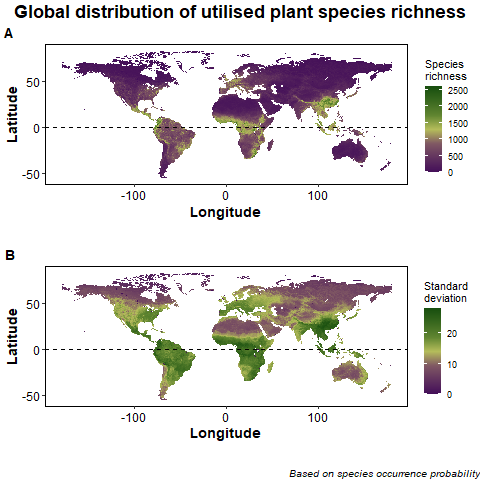
\includegraphics[width=6.67in]{SR_SD} \end{center}

\hypertarget{step-4-computing-the-weighted-endemism-we}{%
\section{\texorpdfstring{Step 4: Computing the weighted endemism
\emph{WE}}{Step 4: Computing the weighted endemism WE}}\label{step-4-computing-the-weighted-endemism-we}}

We apply equations (3) and (4) on \texttt{species\_proba\_per\_cell}.

\begin{Shaded}
\begin{Highlighting}[]

\CommentTok{\# compute the range size weights}
\NormalTok{weights }\OtherTok{\textless{}{-}}\NormalTok{ species\_proba\_per\_cell[, }\FunctionTok{list}\NormalTok{(}\AttributeTok{weight=}\DecValTok{1}\SpecialCharTok{/}\FunctionTok{sum}\NormalTok{(proba,}\AttributeTok{na.rm=}\NormalTok{T)), by}\OtherTok{=}\NormalTok{species]}
\NormalTok{data.table}\SpecialCharTok{::}\FunctionTok{setkey}\NormalTok{(species\_proba\_per\_cell, }\AttributeTok{key=}\StringTok{\textquotesingle{}species\textquotesingle{}}\NormalTok{)}

\CommentTok{\# left join the range size weights to the species probability per cell data}
\NormalTok{species\_proba\_per\_cell[weights, weight}\SpecialCharTok{:}\ErrorTok{=}\NormalTok{weight]}
\FunctionTok{gc}\NormalTok{() }\CommentTok{\# optional, to force R to free some memory for computations}
\NormalTok{data.table}\SpecialCharTok{::}\FunctionTok{setkey}\NormalTok{(species\_proba\_per\_cell, }\AttributeTok{key=}\StringTok{\textquotesingle{}cell\textquotesingle{}}\NormalTok{)}
\FunctionTok{gc}\NormalTok{()}

\CommentTok{\# compute the weighted endemism}
\NormalTok{weighted\_endemism }\OtherTok{\textless{}{-}}\NormalTok{ species\_proba\_per\_cell[,}\FunctionTok{list}\NormalTok{(}\AttributeTok{WE=}\FunctionTok{sum}\NormalTok{(proba}\SpecialCharTok{*}\NormalTok{weight,}\AttributeTok{na.rm=}\NormalTok{T)),}
\NormalTok{                                            by}\OtherTok{=}\NormalTok{cell]}

\CommentTok{\# get valid cell numbers (i.e. cells with values)}
\NormalTok{valid.cells }\OtherTok{\textless{}{-}} \SpecialCharTok{!}\FunctionTok{is.na}\NormalTok{(weighted\_endemism[[}\StringTok{\textquotesingle{}cell\textquotesingle{}}\NormalTok{]])}

\CommentTok{\# create an empty raster to accomodate the weighted endemism estimate}
\NormalTok{predicted\_weighted\_endemism }\OtherTok{\textless{}{-}}\NormalTok{ rast\_ref}

\CommentTok{\# make sure to mask out the original values}
\NormalTok{raster}\SpecialCharTok{::}\FunctionTok{values}\NormalTok{(predicted\_weighted\_endemism) }\OtherTok{\textless{}{-}} \ConstantTok{NA} 

\CommentTok{\# fill up raster values with corresponding estimates}
\NormalTok{predicted\_weighted\_endemism[predicted\_weighted\_endemism[[}\StringTok{\textquotesingle{}cell\textquotesingle{}}\NormalTok{]][valid.cells]] }\OtherTok{\textless{}{-}} 
\NormalTok{  predicted\_weighted\_endemism[[}\StringTok{\textquotesingle{}WE\textquotesingle{}}\NormalTok{]][valid.cells]}
\end{Highlighting}
\end{Shaded}

\begin{Shaded}
\begin{Highlighting}[]

\NormalTok{m }\OtherTok{\textless{}{-}}\NormalTok{ raster}\SpecialCharTok{::}\FunctionTok{rasterToPoints}\NormalTok{(predicted\_weighted\_endemism) }\SpecialCharTok{\%\textgreater{}\%}
  \FunctionTok{as.data.frame}\NormalTok{()}

\NormalTok{weplt }\OtherTok{\textless{}{-}}\NormalTok{ m2 }\SpecialCharTok{\%\textgreater{}\%}
\NormalTok{  ggplot2}\SpecialCharTok{::}\FunctionTok{ggplot}\NormalTok{() }\SpecialCharTok{+}
\NormalTok{  ggplot2}\SpecialCharTok{::}\FunctionTok{geom\_raster}\NormalTok{(ggplot2}\SpecialCharTok{::}\FunctionTok{aes}\NormalTok{(}\AttributeTok{x=}\NormalTok{x,}\AttributeTok{y=}\NormalTok{y,}\AttributeTok{fill=}\FunctionTok{log}\NormalTok{(WE}\SpecialCharTok{+}\DecValTok{1}\NormalTok{))) }\SpecialCharTok{+}
\NormalTok{  ggplot2}\SpecialCharTok{::}\FunctionTok{theme\_classic}\NormalTok{() }\SpecialCharTok{+}
\NormalTok{  ggplot2}\SpecialCharTok{::}\FunctionTok{xlab}\NormalTok{(}\StringTok{"Longitude"}\NormalTok{) }\SpecialCharTok{+}\NormalTok{ ggplot2}\SpecialCharTok{::}\FunctionTok{ylab}\NormalTok{(}\StringTok{"Latitude"}\NormalTok{) }\SpecialCharTok{+}
\NormalTok{  ggplot2}\SpecialCharTok{::}\FunctionTok{labs}\NormalTok{(}\AttributeTok{title=}\StringTok{"Global distribution of useful plant species endemism"}\NormalTok{,}
                \AttributeTok{subtitle =} \StringTok{"based on species occurrence probability"}\NormalTok{) }\SpecialCharTok{+}
\NormalTok{  ggplot2}\SpecialCharTok{::}\FunctionTok{theme}\NormalTok{(}
    \AttributeTok{text=}\NormalTok{ggplot2}\SpecialCharTok{::}\FunctionTok{element\_text}\NormalTok{(}\AttributeTok{family=}\NormalTok{my\_font\_family),}
    \AttributeTok{plot.title =}\NormalTok{ ggplot2}\SpecialCharTok{::}\FunctionTok{element\_text}\NormalTok{(}\AttributeTok{face=}\StringTok{"bold"}\NormalTok{, }\AttributeTok{size=}\DecValTok{18}\NormalTok{, }\AttributeTok{hjust =} \DecValTok{0}\NormalTok{),}
    \AttributeTok{axis.text=}\NormalTok{ggplot2}\SpecialCharTok{::}\FunctionTok{element\_text}\NormalTok{(}\AttributeTok{colour=}\StringTok{"black"}\NormalTok{, }\AttributeTok{size=}\DecValTok{12}\NormalTok{),}
    \AttributeTok{axis.title=}\NormalTok{ggplot2}\SpecialCharTok{::}\FunctionTok{element\_text}\NormalTok{(}\AttributeTok{colour=}\StringTok{"black"}\NormalTok{, }\AttributeTok{size=}\DecValTok{14}\NormalTok{,}\AttributeTok{face=}\StringTok{"bold"}\NormalTok{),}
    \AttributeTok{panel.background =}\NormalTok{ ggplot2}\SpecialCharTok{::}\FunctionTok{element\_rect}\NormalTok{(}\AttributeTok{fill=}\ConstantTok{NA}\NormalTok{, }\AttributeTok{color=}\StringTok{"black"}\NormalTok{, }\AttributeTok{linewidth=}\FloatTok{0.5}\NormalTok{)}
\NormalTok{  )}\SpecialCharTok{+}
\NormalTok{  ggplot2}\SpecialCharTok{::}\FunctionTok{geom\_hline}\NormalTok{(}\AttributeTok{yintercept=}\DecValTok{0}\NormalTok{,}\AttributeTok{linetype=}\StringTok{"dashed"}\NormalTok{) }\SpecialCharTok{+}
\NormalTok{  ggplot2}\SpecialCharTok{::}\FunctionTok{scale\_fill\_viridis\_c}\NormalTok{(}\AttributeTok{name=}\StringTok{\textquotesingle{}Log weighted}\SpecialCharTok{\textbackslash{}n}\StringTok{endemism\textquotesingle{}}\NormalTok{,}
                                \AttributeTok{option=}\StringTok{"magma"}\NormalTok{,}
                                \AttributeTok{direction=}\SpecialCharTok{{-}}\DecValTok{1}\NormalTok{) }\SpecialCharTok{+}
\NormalTok{  ggplot2}\SpecialCharTok{::}\FunctionTok{coord\_equal}\NormalTok{()}

\NormalTok{weplt}
\end{Highlighting}
\end{Shaded}

\begin{center}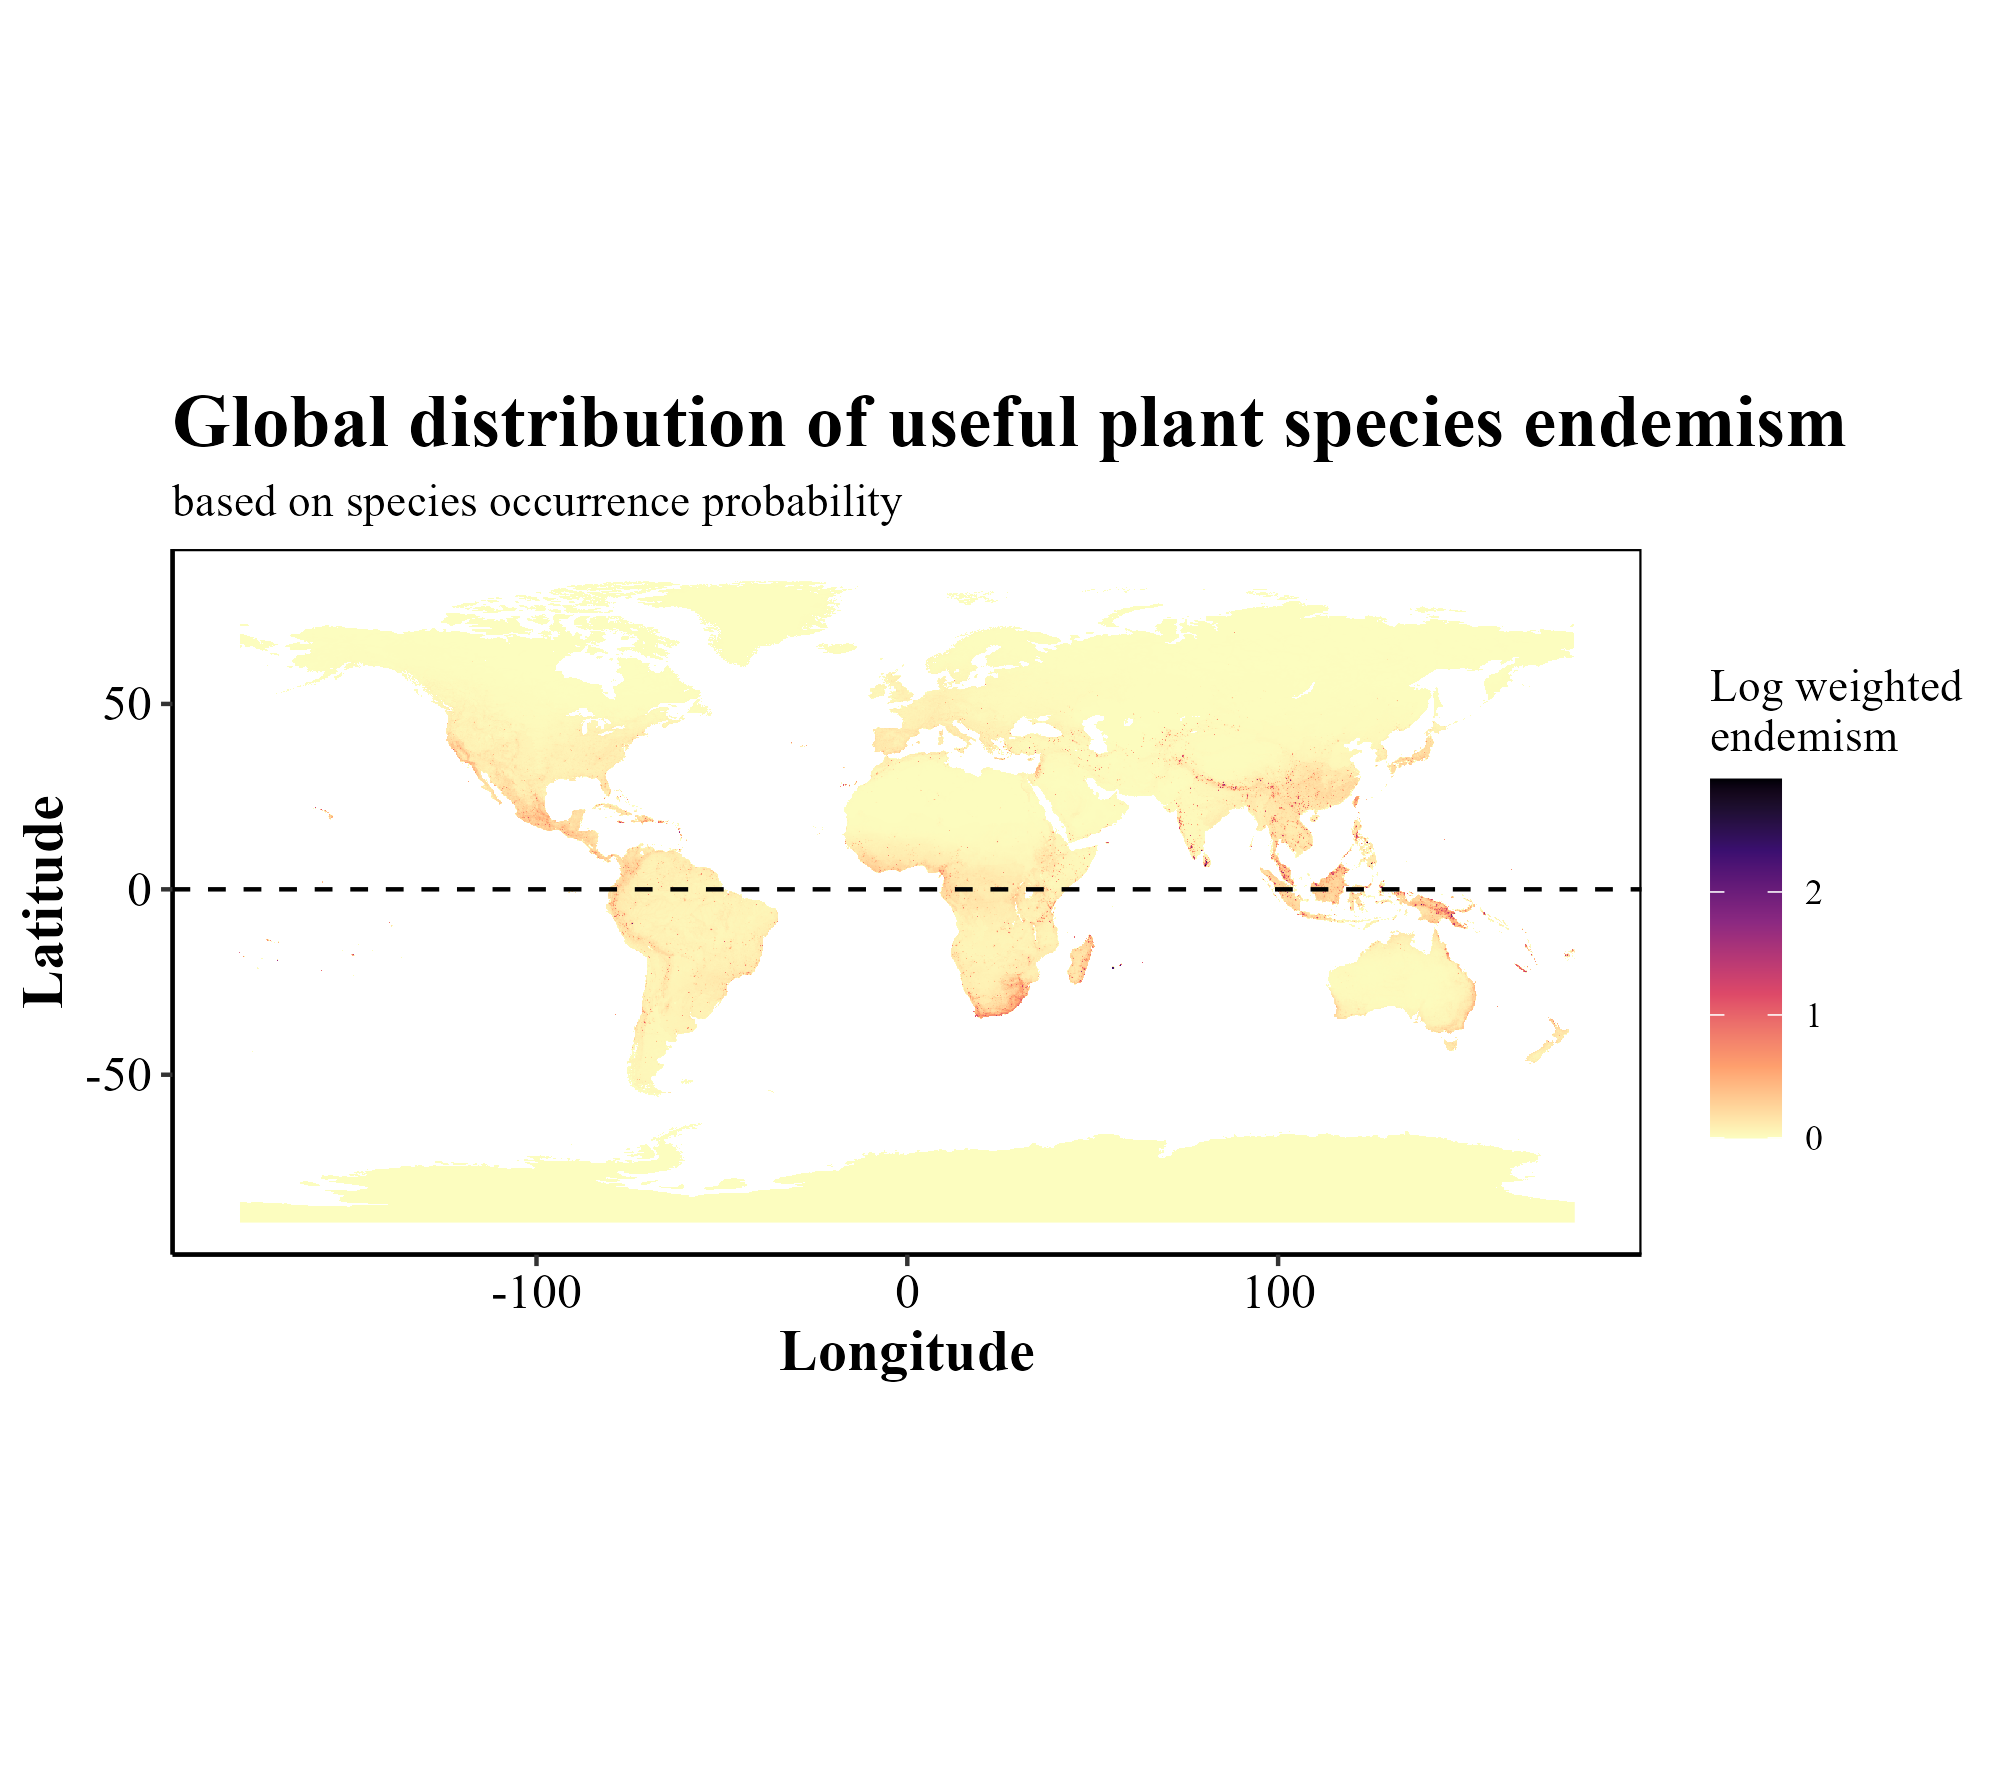
\includegraphics[width=27.9in]{WE} \end{center}

\hypertarget{references}{%
\section*{References}\label{references}}
\addcontentsline{toc}{section}{References}

\hypertarget{refs}{}
\begin{CSLReferences}{1}{0}
\leavevmode\vadjust pre{\hypertarget{ref-Calabrese2014}{}}%
Calabrese, Justin M., Grégoire Certain, Casper Kraan, and Carsten F.
Dormann. 2014. {``Stacking Species Distribution Models and Adjusting
Bias by Linking Them to Macroecological Models.''} \emph{Global Ecology
and Biogeography} 23 (1): 99--112.
https://doi.org/\url{https://doi.org/10.1111/geb.12102}.

\leavevmode\vadjust pre{\hypertarget{ref-crisp2001endemism}{}}%
Crisp, MICHAEL D, Shawn Laffan, H Peter Linder, and ANNA Monro. 2001.
{``Endemism in the Australian Flora.''} \emph{Journal of Biogeography}
28 (2): 183--98.

\leavevmode\vadjust pre{\hypertarget{ref-data_table}{}}%
Dowle, Matt, and Arun Srinivasan. 2021. \emph{Data.table: Extension of
`Data.frame`}. \url{https://CRAN.R-project.org/package=data.table}.

\leavevmode\vadjust pre{\hypertarget{ref-terra}{}}%
Hijmans, Robert J. 2023. \emph{Terra: Spatial Data Analysis}.
\url{https://CRAN.R-project.org/package=terra}.

\leavevmode\vadjust pre{\hypertarget{ref-ggpubr}{}}%
Kassambara, Alboukadel. 2023. \emph{Ggpubr: 'Ggplot2' Based Publication
Ready Plots}. \url{https://CRAN.R-project.org/package=ggpubr}.

\leavevmode\vadjust pre{\hypertarget{ref-UsefulPlants}{}}%
Pironon S., Diazgranados M., Ondo I. 2023. {``The Global Distribution of
Plants Used by Humans.''} Journal Article.

\leavevmode\vadjust pre{\hypertarget{ref-ggplot2}{}}%
Wickham, Hadley. 2016. \emph{Ggplot2: Elegant Graphics for Data
Analysis}. Springer-Verlag New York.
\url{https://ggplot2.tidyverse.org}.

\end{CSLReferences}

\end{document}
